\documentclass[border=4pt]{standalone}
\usepackage{tikz}
\usetikzlibrary{arrows.meta,shapes.geometric}
\begin{document}
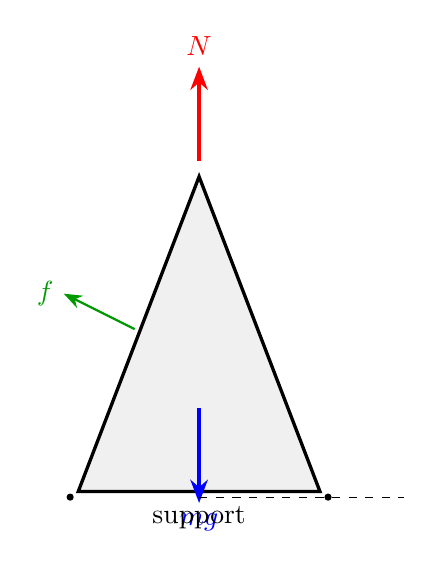
\begin{tikzpicture}[>=Stealth]
  \node[
    isosceles triangle,
    isosceles triangle apex angle=42,
    shape border rotate=90,
    minimum height=4cm,
    inner sep=0pt,
    anchor=lower side,
    draw=black,
    very thick,
    fill=gray!12,
    outer sep=2pt
  ] (wedge) at (0,0) {};
  \fill (wedge.left corner) circle (1.3pt);
  \fill (wedge.right corner) circle (1.3pt);
  \draw[->,red,very thick] (wedge.apex) -- ++(0,1.2) node[above] {$N$};
  \draw[->,blue,very thick] (wedge.center) -- ++(0,-1.2) node[below] {$mg$};
  \draw[->,green!60!black,thick] (wedge.left side) -- ++(-0.9,0.45) node[left] {$f$};
  \draw[dashed] (wedge.lower side) -- ++(2.6,0);
  \node[below] at (wedge.lower side) {support};
\end{tikzpicture}
\end{document}
